
\documentclass[letterpaper]{article}
\usepackage{underscore}
\usepackage[left=2.0cm, right=2.0cm, top=2.0cm]{geometry}
\usepackage[utf8]{inputenc}
\usepackage{graphicx}
\usepackage{graphics}
\usepackage[spanish]{babel}
\usepackage{lipsum}
\usepackage{float}
\usepackage{subfigure}

\title{EV\_2\_2\_Explicar\_los\_arreglos\_y\_parámetros\\\_de\_los\_amplificadores\_clase\_A}
\author{Alcantar Diaz Joel Alejandro.}
\date{24/09/2019}

\begin{document}

    \maketitle
    \begin{center}
        
\includegraphics[scale=0.5]{IMG/UPZMGlog.png}\\
        \vspace{2cm}
    \textbf{Univercidad Politécnica de la Zona Metropolitana de Guadalajara $|$ Ing. Mecatrónica 4$^{to}$ $"$A$"$}
    \end{center}
    \newpage
    \begin{large}
        \begin{center}
            \textbf{¿Como funciona un amplificador de clase A?}
        \end{center}
        Los amplificadores de clase A son en pocas palabras los mas eficientes a la hora de amplificar, ya que la fidelidad de estos es la mas alta. Si se le mete una señal de, por ejemplo, 5 volts el trancistor nos dara una señal igual pero amplificada a un maximo de la tencion de la fuente, esto se puede ver mejor en las señales senoidales ya que su voltaje pico pico se amplia.\\\\
        Las desventajas que tienen estos amplificadores es que consumen mucha corriente aun estando en desuso y su eficiencia es tambien muy poca llegando solo al 30\%. Si por ejemplo,se tiene que el transistor consume 100 ampers, de ellos solo aprebechara 30 y los otros 70 seran desechados en enegia calorica. Es por ello que se requiere constante dicipacion en los tancistores ya que entre mas caliente menos eficeinte sera.\\\\
        \begin{center}
            \textbf{Configuraciones de amplificadores clase A: Amplificador de uan sola etapa.}
        \end{center}
        Este es el mas simple de los circuitos de amplificacion de clase A. Solo utiliza un trancistor para la salida con una resitencia conectada al colector. Cuando el trancistor esta activo la corriente cae en el lo que resulta en una caida de tencion a traves de la resistencia del emisor y asi limitando la salida negativa. Precisamente en este circuito es donde la eficiencia es la menor ya que la corriente que pasa es la misma incluso si no tiene señal de entrada.\\\\
        \begin{figure}[htbp]
            \centering
            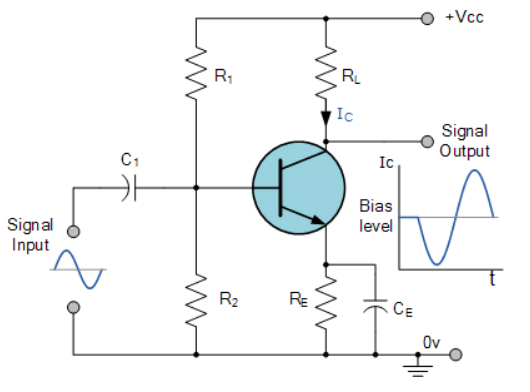
\includegraphics[scale=0.5]{IMG/cir1.jpg}
            \caption{Circuito amplificador de una sola etapa.}
            \label{fig:cir1}
        \end{figure}
        \newpage
        \begin{center}
            \textbf{Amplificador con trancistor Darlington.}
        \end{center}
        Este tipo de dispositivos son basicamente 2 trancistores dentro de un solo empaquetado. Contiene un trancistor al que se le llama piloto y otro de comutacion mas grande. La ventaja es que la inpedancia de salida es muy baja y la de entrada es adecuadamente grande.\\\\
        La ganancia de hfe ($\beta$) de estos trancistores es el producto de las 2 ganancias individuales de los trancistores.\\\\
        \begin{figure}[htbp]
            \centering
            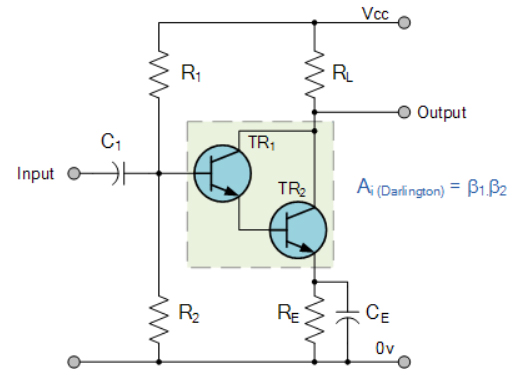
\includegraphics[scale=0.5]{IMG/cir2.jpg}
            \caption{Amplificador con Darlington.}
            \label{fig:cir2}
        \end{figure}
        \begin{center}
            \textbf{Amplificador acoplado a transformador}
        \end{center}
        En este circuito el tranformador mejora la eficiencia del amplificador al hacer coincidir la impedancia de la carga con la de salida utilizando la relacion de vueltas de un transformador.\\\\
        En este circuito el flujo magnetico del tranformador en el nucluo colapsa causando una fem inducida en los devanados primarios. Esto hace que la tencion en el colector aumente al doble de la tencion de alimentacion en el colector.
        \begin{figure}[htbp]
            \centering
            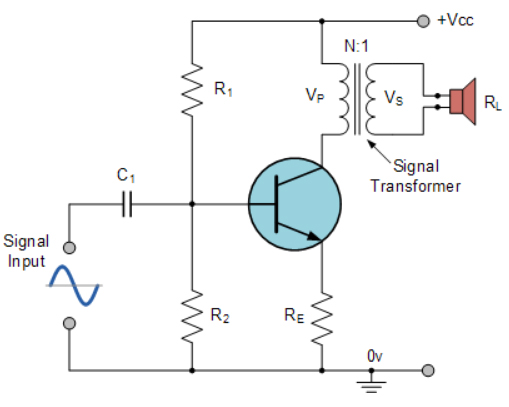
\includegraphics[scale=0.5]{IMG/cir3.jpg}
            \caption{Amplificador acoplado a transformador}
            \label{fig:cir3}
        \end{figure}
        \newpage
    \end{large}
    \begin{thebibliography}{X}
    \bibitem{1} \textit{Amplificador de potencia: CLASE A[Archivo de video].} (2018, 17 mayo). Recuperado 1 octubre, 2019, de https://www.youtube.com/watch?v=1\_7FNawxMEA
    \bibitem{2} \textit{Amplificadores de potencia: casificaión, clase A, B, AB, C - Electronica Unicrom.} (2018, 9 noviembre). Recuperado 1 octubre, 2019, de https://unicrom.com/amplificadores-de-potencia-clasificacion/
    \bibitem{3} \textit{Clases de amplificador y la clasificacion de amplificadores. (s.f.).} Recuperado 1 octubre, 2019, de http://tutorialesdeelectronicabasica.blogspot.com/2018/06/clases-de-amplificador-y-la.html
    \bibitem{4} \textit{El amplificador de clase A es un amplificador de trancistor de clase A. (s.f.)} Recuperado 1 octubre, 2019, de http://tutorialesdeelectronicabasica.blogspot.com/2018/06/el-amplificador-de-clase-es-un.html
    \end{thebibliography}
\end{document}